% 建议使用 XeLaTeX 或 LuaLaTeX 编译(中文与公式支持更佳)
\documentclass[UTF8,zihao=-4]{ctexart}

\usepackage[a4paper,margin=2.5cm]{geometry}
\usepackage{amsmath, amssymb, amsthm}
\usepackage{bm}
\usepackage{hyperref}
\usepackage{graphicx}
\usepackage{caption}
\usepackage{listings}
\usepackage{xcolor}
\usepackage{float}
\usepackage{placeins}
\graphicspath{{figures/}}

\lstdefinestyle{code}{
  basicstyle=\ttfamily\small,
  numbers=left,
  numberstyle=\tiny,
  numbersep=8pt,
  keywordstyle=\color{blue},
  commentstyle=\color{teal!70!black},
  stringstyle=\color{orange!70!black},
  showstringspaces=false,
  breaklines=true,
  frame=single,
  framerule=0.3pt,
  rulecolor=\color{black!15}
}
\lstset{style=code}

\title{软演员-评论家(SAC):原理、公式、应用与实战}
\author{}
\date{\today}

\begin{document}
\maketitle

\section{引言}
软演员-评论家(Soft Actor-Critic,SAC)在最大熵框架下同时最大化期望回报与策略熵,通过双 Q 网络、随机策略与自适应温度,实现连续控制任务中的高性能与稳定性。

\section{原理与公式}
\subsection{最大熵目标}
SAC 优化目标为:
\begin{equation}
J(\pi) = \mathbb{E}_{\tau \sim \pi}\Big[ \sum_{t} \gamma^t (r_{t+1} + \alpha \mathcal{H}(\pi(\cdot\mid s_t))) \Big],
\end{equation}
其中 \(\alpha\) 权衡奖励与熵。

\subsection{评论家与策略更新}
双 Q 网络 \(Q_{w_i}\) 最小化:
\begin{equation}
L(w_i) = \mathbb{E}\Big[(Q_{w_i}(s,a) - y)^2\Big], \quad y = r + \gamma (\min_j Q_{w_j^-}(s', a') - \alpha \log \pi_\theta(a'\mid s')).
\end{equation}
策略通过重参数化技巧更新:
\begin{equation}
\nabla_\theta J_{\pi} = \mathbb{E}_{s,\varepsilon}\big[ \nabla_\theta \alpha \log \pi_\theta(f_\theta(\varepsilon; s)\mid s) - \nabla_\theta Q_{w_1}(s, f_\theta(\varepsilon; s)) \big].
\end{equation}

\subsection{温度自适应}
温度 \(\alpha\) 通过最小化:
\begin{equation}
J(\alpha) = \mathbb{E}_{a \sim \pi_\theta}\big[ -\alpha (\log \pi_\theta(a\mid s) + \mathcal{H}_{\text{target}}) \big],
\end{equation}
自动调整熵水平,平衡探索与利用。

\section{应用与技巧}
\begin{itemize}
  \item \textbf{连续控制}:广泛用于机器人、自动驾驶等场景。
  \item \textbf{采样效率}:结合经验回放的离策略更新极具效率。
  \item \textbf{策略鲁棒性}:最大熵目标鼓励多样化动作。
  \item \textbf{实用建议}:规范化观测、保持双 Q 网络、使用对数参数化的 \(\alpha\)、监控熵与 critic 损失。
\end{itemize}

\section{Python 实战}
脚本 \texttt{gen\_sac\_figures.py} 在一维连续控制任务中实现简化版 SAC,记录回报曲线与温度参数的变化趋势。
\begin{lstlisting}[language=Python,caption={脚本 gen_sac_figures.py 片段}]
q_target = reward + gamma * (min_q_target - alpha * log_prob_next)
critic_w1 += critic_lr * (q_target - q1) * features(state, action)
critic_w2 += critic_lr * (q_target - q2) * features(state, action)

alpha_grad = -np.mean(log_prob + target_entropy)
log_alpha += alpha_lr * alpha_grad
alpha = np.exp(log_alpha)
\end{lstlisting}

\section{实验结果}
\begin{figure}[H]
  \centering
  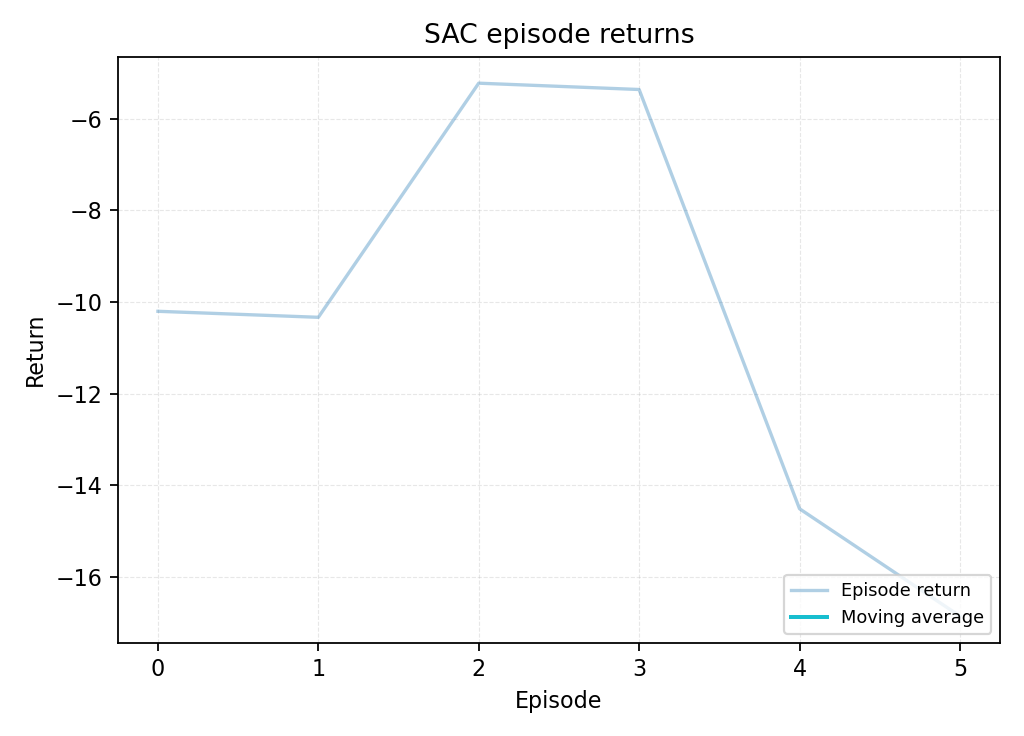
\includegraphics[width=0.8\linewidth]{sac_returns.png}
  \caption{SAC 训练回报的稳步提升}
  \label{fig:sac_returns_cn}
\end{figure}

\begin{figure}[H]
  \centering
  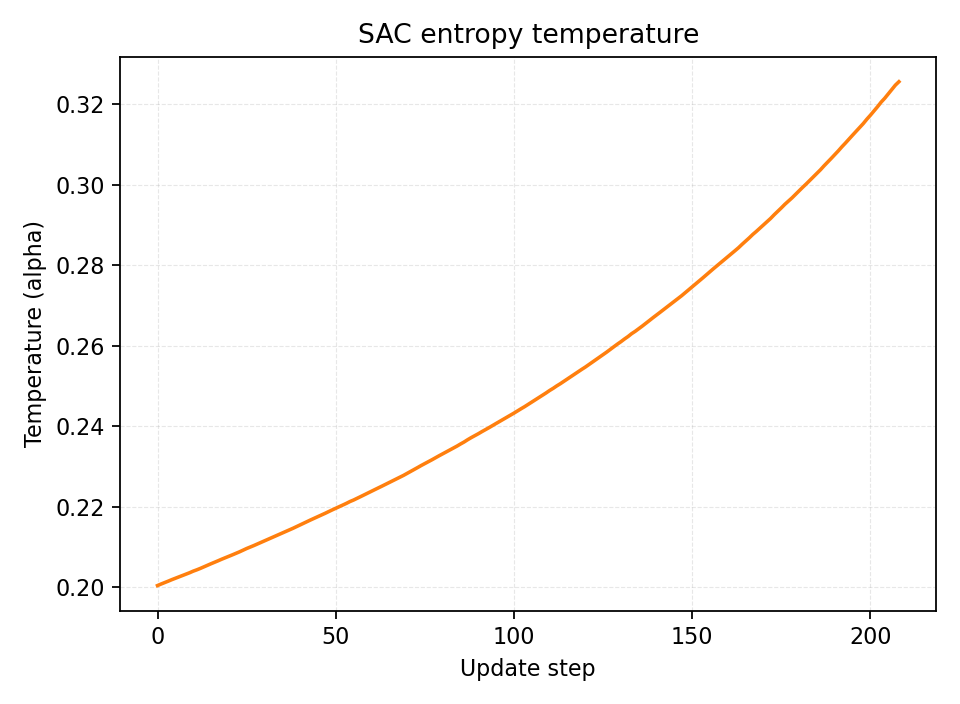
\includegraphics[width=0.82\linewidth]{sac_temperature.png}
  \caption{温度参数收敛至目标熵附近}
  \label{fig:sac_temperature_cn}
\end{figure}

\FloatBarrier
\section{总结}
SAC 通过双 Q 网络、随机策略与温度自适应实现稳定高效的连续控制学习。恰当的归一化、经验管理与熵监控可显著提升性能。示例展示了回报提升及温度动态符合预期。

\end{document}